\documentclass[a0paper,portrait]{baposter}

\usepackage{lmodern}
\usepackage[utf8]{inputenc}
\usepackage[T1]{fontenc}
\usepackage{booktabs}
\usepackage{multirow}
\usepackage{graphicx}
\usepackage{colortbl}

\usepackage{tikz}
\usetikzlibrary{shadows, positioning, fit}

\usepackage{amssymb}
\usepackage{comment}


\selectcolormodel{cmyk}

\graphicspath{{figures/}}

\newcommand{\compresslist}{%
\setlength{\itemsep}{0pt}%
\setlength{\parskip}{1pt}%
\setlength{\parsep}{0pt}%
}

\newenvironment{boenumerate}
  {\begin{enumerate}\renewcommand\labelenumi{\textbf\theenumi.}}
  {\end{enumerate}}

\begin{document}

\definecolor{darkblue}{cmyk}{1,0.5,0,0.3}
\definecolor{lightblue}{cmyk}{0.5,0.2,0,0.1}
\definecolor{lightlightblue}{cmyk}{0.15,0,0,0.02}

\begin{poster}
{
grid=false,
headerborder=open,
colspacing=1em,
bgColorOne=lightlightblue,
bgColorTwo=lightlightblue,
borderColor=darkblue,
headerColorOne=lightblue,
headerColorTwo=lightblue,
headerFontColor=white,
boxColorOne=white,
textborder=rounded,
eyecatcher=false,
headerheight=0.11\textheight,
headershape=rounded,
headershade=plain,
headerfont=\Large\textsf,
linewidth=2pt
}
{}
{
 \LARGE \textsf{Building Predictive Models through Human-Guided Machine Learning: A Tool for Non-Experts}
}
{\sf\vspace{0.5em}\\
Diego García-Prieto*, Camilo Palazuelos, Rafael Duque
\vspace{0.1em}\\
\small{Department of Mathematics, Statistics and Computer Science, University of Cantabria, Spain
\vspace{0.2em}\\
diego.garciaprieto@unican.es, camilo.palazuelos@unican.es, rafael.duque@unican.es}
}
{
\includegraphics[width=0.25\linewidth]{figures/UC_LogotipoPrincipal.png}}

\headerbox{1. Motivation}{name=motivation,column=0,row=0,span=3}{
Current AutoML tools prioritize \textbf{automation} over \textbf{human control}, creating ``black boxes'' that exclude domain expertise and limit transparency

\vspace{5pt}
``Interactive Support for Non-Expert Users in Machine Learning'' (\textbf{InsuML}) bridges this gap by implementing Human-Guided Machine Learning (HGML) principles, keeping a \textbf{human-in-the-loop} approach that lets non-AI experts guide to build predictive models through intuitive interfaces while maintaining oversight across the ML pipeline
}

\headerbox{2. The Problem}{name=problem,column=0,below=motivation,span=1}{
\textbf{Traditional AutoML Limitations:}
\begin{itemize}\compresslist
    \item Opaque decision-making
    \item Limited domain knowledge integration
    \item Insufficient interpretability
    \item Risk of bias propagation
    \item Expert-only accessibility
\end{itemize}

\vspace{5pt}
\textbf{Human-Centered AI Framework:}
\begin{center}
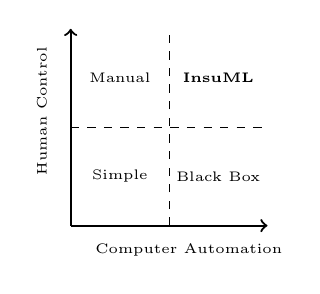
\begin{tikzpicture}[scale=0.5]
    \draw[->, thick] (0,0) -- (5,0) node[anchor=north, xshift=-1cm, yshift=-3pt, font=\tiny] {Computer Automation};
    \draw[->, thick] (0,0) -- (0,5) node[anchor=south east, rotate=90, xshift=-3pt, yshift=5pt, font=\tiny] {Human Control};
    \draw[dashed] (0,2.5) -- (5,2.5);
    \draw[dashed] (2.5,0) -- (2.5,5);
    
    \node[align=center, font=\tiny] at (1.25,1.25) {Simple};
    \node[align=center, font=\tiny] at (3.75,1.25) {Black Box};
    \node[align=center, font=\tiny] at (1.25,3.75) {Manual};
    \node[align=center, font=\tiny] at (3.75,3.75) {\textbf{InsuML}};
\end{tikzpicture}
\end{center}
}

\headerbox{3. AutoML Comparison}{name=automl,column=1,below=motivation,span=2}{

{\scriptsize
\renewcommand{\arraystretch}{1.2}
\begin{center}
\resizebox{0.9\linewidth}{!}{
\begin{tabular}{c c c c | c c c c c c}
\toprule
\multirow{3}{*}{\textbf{\begin{tabular}{@{}c@{}} AutoML \\ tool \end{tabular}}} 
  & \multicolumn{9}{c}{\textbf{HCAI Framework}} \\ \cmidrule(lr){2-10}
  & \multicolumn{3}{c|}{\textbf{Human Control}} 
  & \multicolumn{6}{c}{\textbf{High Automation}} \\ \cmidrule(lr){2-4} \cmidrule(lr){5-10}
  & \textbf{\begin{tabular}{@{}c@{}} Easy-to-use \end{tabular}} 
  & \textbf{\begin{tabular}{@{}c@{}} Configurable \\ pipeline \end{tabular}} 
  & \textbf{\begin{tabular}{@{}c@{}} Interpretable \\ information \end{tabular}} 
  & \textbf{\begin{tabular}{@{}c@{}} Data \\ types \end{tabular}} 
  & \textbf{\begin{tabular}{@{}c@{}} Data \\ cleaning \end{tabular}} 
  & \textbf{\begin{tabular}{@{}c@{}} Feature \\ engineering \end{tabular}} 
  & \textbf{\begin{tabular}{@{}c@{}} Model \\ training \end{tabular}} 
  & \textbf{\begin{tabular}{@{}c@{}} Hyperparameter \\ tuning \end{tabular}} 
  & \textbf{\begin{tabular}{@{}c@{}} Model \\ validation \end{tabular}} \\ \midrule
\textbf{MindsDB} & Medium & Low & Medium & \checkmark & \checkmark & \checkmark & \checkmark & \checkmark & \checkmark \\
\textbf{Prophet} & Low & Medium & Medium &  & \checkmark &  & \checkmark & \checkmark & \checkmark \\
\textbf{NNI} & Medium & High & Medium &  &  & \checkmark & \checkmark & \checkmark & \checkmark \\
\textbf{H2O-3} & Medium & High & Medium & \checkmark & \checkmark & \checkmark & \checkmark & \checkmark & \checkmark \\
\textbf{Ludwig} & Medium & High & Medium & \checkmark & \checkmark & \checkmark & \checkmark & \checkmark & \checkmark \\
\textbf{Optuna} & Low & High & Medium &  &  &  & \checkmark & \checkmark & \checkmark \\
\textbf{PyCaret} & Low & High & Medium & \checkmark & \checkmark & \checkmark & \checkmark & \checkmark & \checkmark \\
\textbf{TPOT} & Low & High & Low & \checkmark &  & \checkmark & \checkmark & \checkmark & \checkmark \\
\textbf{AutoKeras} & Low & High & Low &  &  &  & \checkmark & \checkmark & \checkmark \\
\textbf{AutoGluon} & Medium & High & Medium & \checkmark & \checkmark & \checkmark & \checkmark & \checkmark & \checkmark \\
\textbf{Hyperopt} & Low & High & Low &  &  &  & \checkmark & \checkmark &  \\
\textbf{Featuretools} & Low & Medium & Low &  &  & \checkmark &  &  &  \\
\textbf{Auto-Sklearn} & Low & High & Low & \checkmark & \checkmark & \checkmark & \checkmark & \checkmark & \checkmark \\ 
\bottomrule
\end{tabular}
}
\end{center}
}

No single tool simultaneously maximizes both human control and automation
}


\headerbox{4. System Architecture}{name=architecture,column=0,below=problem,span=1}{

\centering
\scalebox{0.63}{
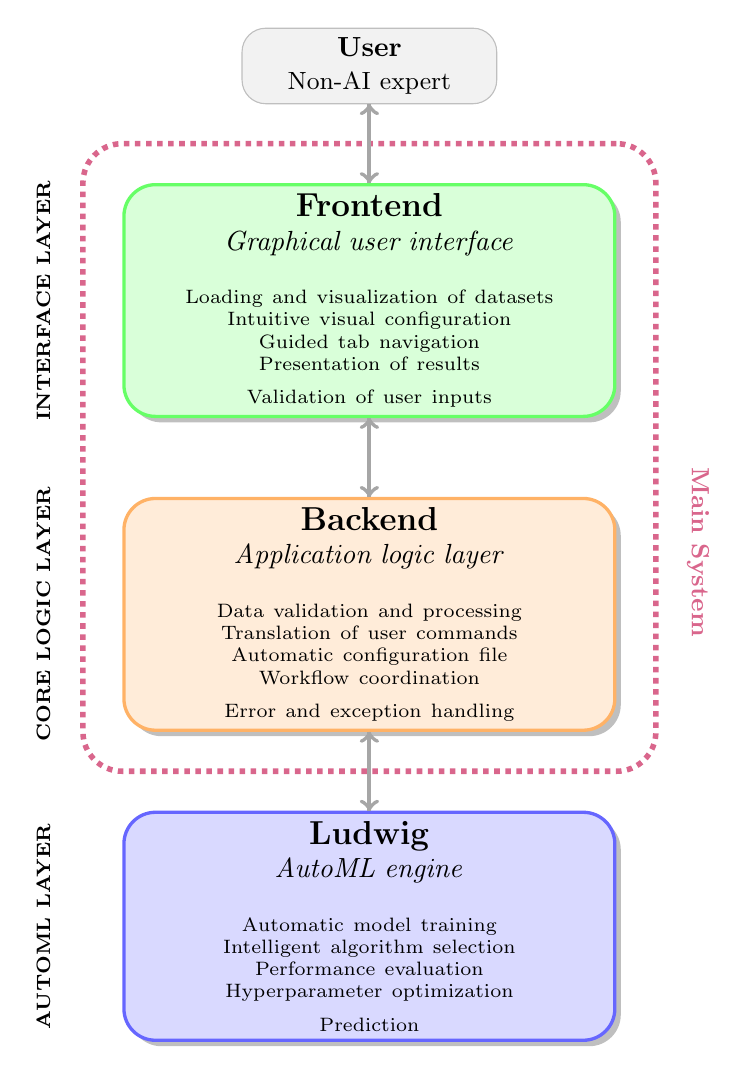
\begin{tikzpicture}[
    node distance=3.5cm,
    box/.style={
        rectangle,
        draw,
        text width=6cm,
        text centered,
        minimum height=2.8cm,
        rounded corners=0.4cm,
        drop shadow,
        line width=1.2pt
    },
    frontend/.style={box, fill=green!15, draw=green!60},
    backend/.style={box, fill=orange!15, draw=orange!60},
    ludwig/.style={box, fill=blue!15, draw=blue!60},
    arrow/.style={->, thick, color=gray!70, line width=1.5pt},
    label/.style={font=\small\bfseries, color=gray!80},
    system/.style={
        rectangle,
        draw,
        dotted,
        thick,
        rounded corners=0.5cm,
        color=purple!60,
        line width=2pt
    }
]
% Nodos principales (disposición vertical)
\node[frontend] (frontend) {
    \textbf{\large Frontend}\\
    \textit{Graphical user interface}\\[0.4cm]
    \scriptsize{
        Loading and visualization of datasets\\
        Intuitive visual configuration\\
        Guided tab navigation\\
        Presentation of results\\
        Validation of user inputs
    }
};
\node[backend, below=1cm of frontend] (backend) {
    \textbf{\large Backend}\\
    \textit{Application logic layer}\\[0.4cm]
    \scriptsize{
        Data validation and processing\\
        Translation of user commands\\
        Automatic configuration file\\
        Workflow coordination\\
        Error and exception handling
    }
};
\node[ludwig, below=1cm of backend] (ludwig) {
    \textbf{\large Ludwig}\\
    \textit{AutoML engine}\\[0.4cm]
        \scriptsize{
        Automatic model training\\
        Intelligent algorithm selection\\
        Performance evaluation\\
        Hyperparameter optimization\\
        Prediction
    }
};

% Rectángulo punteado alrededor de Frontend y Backend
\node[system, fit=(frontend)(backend), inner sep=0.5cm] (main_system) {};

% Etiqueta del sistema
\node[right=0.5cm of main_system.east, 
      font=\small\bfseries, 
      color=purple!60,
      rotate=-90] {Main System};

% Bidirectional arrows
\draw[arrow] (frontend.south) -- (backend.north) node[midway, right] {\label{commands_and_configuration}};
\draw[arrow] (backend.north) -- (frontend.south) node[midway, left] {\label{responses_and_results}};
\draw[arrow] (backend.south) -- (ludwig.north) node[midway, right] {\label{yaml_configuration}};
\draw[arrow] (ludwig.north) -- (backend.south) node[midway, left] {\label{metrics_and_models}};

% Side labels
\node[left=1cm of frontend, rotate=90, anchor=center] {\scriptsize \textbf{INTERFACE LAYER}};
\node[left=1cm of backend, rotate=90, anchor=center] {\scriptsize \textbf{CORE LOGIC LAYER}};
\node[left=1cm of ludwig, rotate=90, anchor=center] {\scriptsize \textbf{AUTOML LAYER}};

% User
\node[above=1cm of frontend, 
      rectangle, 
      draw=gray!50, 
      fill=gray!10, 
      text width=3cm, 
      text centered,
      rounded corners=0.3cm] (user) {
    \textbf{User}\\
    \small{Non-AI expert}
};
\draw[arrow] (user.south) -- (frontend.north) node[midway, right] {\label{Interaction}};
\draw[arrow] (frontend.north) -- (user.south) node[midway, left] {\label{Feedback}};
\end{tikzpicture}
}

\vspace{8pt}
Modular, transparent design enabling AutoML with a user-friendly, interactive interface while preserving HGML principles
}

\headerbox{5. Experimental Results}{name=results,span=2,column=1,below=automl}{

\begin{center}
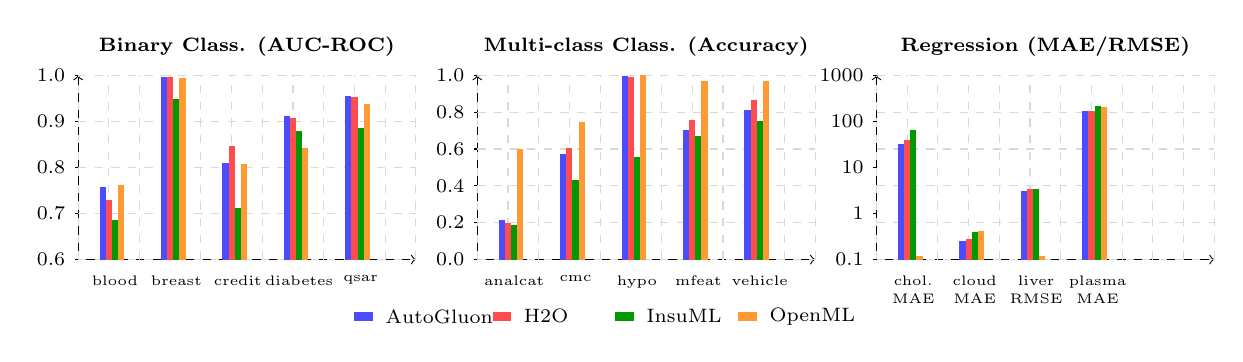
\begin{tikzpicture}[scale=0.39]

% ===== GRÁFICA 1: Binary Classification =====
\begin{scope}[xshift=0cm]
\draw[->] (0,0) -- (0,6) node[above, font=\small] {};
\draw[->] (0,0) -- (11,0);
\draw[dashed, gray!30] (0,0) grid[ystep=1.5] (11,6);

% Escala Y
\foreach \y/\val in {0/0.6, 1.5/0.7, 3/0.8, 4.5/0.9, 6/1.0}
    \draw (0,\y) -- (-0.1,\y) node[left, font=\scriptsize] {\val};

% Etiquetas X
\foreach \x/\name in {1.2/blood, 3.2/breast, 5.2/credit, 7.2/diabetes, 9.2/qsar} {
    \node[below, font=\tiny] at (\x,-0.2) {\name};
}

% Barras - AutoGluon (azul)
\fill[blue!70] (0.7,0) rectangle (0.9,{(0.757-0.6)*15});
\fill[blue!70] (2.7,0) rectangle (2.9,{(0.997-0.6)*15});
\fill[blue!70] (4.7,0) rectangle (4.9,{(0.810-0.6)*15});
\fill[blue!70] (6.7,0) rectangle (6.9,{(0.912-0.6)*15});
\fill[blue!70] (8.7,0) rectangle (8.9,{(0.954-0.6)*15});

% H2O (rojo)
\fill[red!70] (0.9,0) rectangle (1.1,{(0.730-0.6)*15});
\fill[red!70] (2.9,0) rectangle (3.1,{(0.996-0.6)*15});
\fill[red!70] (4.9,0) rectangle (5.1,{(0.847-0.6)*15});
\fill[red!70] (6.9,0) rectangle (7.1,{(0.908-0.6)*15});
\fill[red!70] (8.9,0) rectangle (9.1,{(0.953-0.6)*15});

% InsuML (verde)
\fill[green!60!black] (1.1,0) rectangle (1.3,{(0.686-0.6)*15});
\fill[green!60!black] (3.1,0) rectangle (3.3,{(0.949-0.6)*15});
\fill[green!60!black] (5.1,0) rectangle (5.3,{(0.711-0.6)*15});
\fill[green!60!black] (7.1,0) rectangle (7.3,{(0.878-0.6)*15});
\fill[green!60!black] (9.1,0) rectangle (9.3,{(0.886-0.6)*15});

% OpenML (naranja)
\fill[orange!80] (1.3,0) rectangle (1.5,{(0.761-0.6)*15});
\fill[orange!80] (3.3,0) rectangle (3.5,{(0.995-0.6)*15});
\fill[orange!80] (5.3,0) rectangle (5.5,{(0.807-0.6)*15});
\fill[orange!80] (7.3,0) rectangle (7.5,{(0.843-0.6)*15});
\fill[orange!80] (9.3,0) rectangle (9.5,{(0.938-0.6)*15});

\node[above, font=\scriptsize\bfseries] at (5.5,6.3) {Binary Class. (AUC-ROC)};
\end{scope}

% ===== GRÁFICA 2: Multi-class Classification =====
\begin{scope}[xshift=13cm]
\draw[->] (0,0) -- (0,6) node[above, font=\small] {};
\draw[->] (0,0) -- (11,0);
\draw[dashed, gray!30] (0,0) grid[ystep=1.2] (11,6);

% Escala Y
\foreach \y/\val in {0/0.0, 1.2/0.2, 2.4/0.4, 3.6/0.6, 4.8/0.8, 6/1.0}
    \draw (0,\y) -- (-0.1,\y) node[left, font=\scriptsize] {\val};

% Etiquetas X
\foreach \x/\name in {1.2/analcat, 3.2/cmc, 5.2/hypo, 7.2/mfeat, 9.2/vehicle} {
    \node[below, font=\tiny] at (\x,-0.2) {\name};
}

% Barras - AutoGluon
\fill[blue!70] (0.7,0) rectangle (0.9,{0.213*6});
\fill[blue!70] (2.7,0) rectangle (2.9,{0.574*6});
\fill[blue!70] (4.7,0) rectangle (4.9,{0.995*6});
\fill[blue!70] (6.7,0) rectangle (6.9,{0.705*6});
\fill[blue!70] (8.7,0) rectangle (8.9,{0.812*6});

% H2O
\fill[red!70] (0.9,0) rectangle (1.1,{0.200*6});
\fill[red!70] (2.9,0) rectangle (3.1,{0.604*6});
\fill[red!70] (4.9,0) rectangle (5.1,{0.993*6});
\fill[red!70] (6.9,0) rectangle (7.1,{0.755*6});
\fill[red!70] (8.9,0) rectangle (9.1,{0.867*6});

% InsuML
\fill[green!60!black] (1.1,0) rectangle (1.3,{0.190*6});
\fill[green!60!black] (3.1,0) rectangle (3.3,{0.430*6});
\fill[green!60!black] (5.1,0) rectangle (5.3,{0.558*6});
\fill[green!60!black] (7.1,0) rectangle (7.3,{0.670*6});
\fill[green!60!black] (9.1,0) rectangle (9.3,{0.750*6});

% OpenML
\fill[orange!80] (1.3,0) rectangle (1.5,{0.599*6});
\fill[orange!80] (3.3,0) rectangle (3.5,{0.749*6});
\fill[orange!80] (5.3,0) rectangle (5.5,{0.9995*6});
\fill[orange!80] (7.3,0) rectangle (7.5,{0.970*6});
\fill[orange!80] (9.3,0) rectangle (9.5,{0.970*6});

\node[above, font=\scriptsize\bfseries] at (5.5,6.3) {Multi-class Class. (Accuracy)};
\end{scope}

% ===== GRÁFICA 3: Regression (Escala Logarítmica) =====
\begin{scope}[xshift=26cm]
\draw[->] (0,0) -- (0,6) node[above, font=\small] {};
\draw[->] (0,0) -- (11,0);
\draw[dashed, gray!30] (0,0) grid[ystep=1.2] (11,6);

% Escala Y logarítmica: 0.1, 1, 10, 100
\foreach \y/\val in {0/0.1, 1.5/1, 3/10, 4.5/100, 6/1000}
    \draw (0,\y) -- (-0.1,\y) node[left, font=\scriptsize] {\val};

% Etiquetas X
\foreach \x/\name in {1.2/chol., 3.2/cloud, 5.2/liver, 7.2/plasma} {
    \node[below, font=\tiny] at (\x,-0.2) {\name};
}

% Función logarítmica: (log10(valor) + 1) * 1.5

% cholesterol (MAE)
\fill[blue!70] (0.7,0) rectangle (0.9,{(log10(31.910) + 1) * 1.5});
\fill[red!70] (0.9,0) rectangle (1.1,{(log10(39.729) + 1) * 1.5});
\fill[green!60!black] (1.1,0) rectangle (1.3,{(log10(63.463) + 1) * 1.5});
\fill[orange!80] (1.3,0) rectangle (1.5,{0.1});

% cloud (MAE)
\fill[blue!70] (2.7,0) rectangle (2.9,{(log10(0.254) + 1) * 1.5});
\fill[red!70] (2.9,0) rectangle (3.1,{(log10(0.277) + 1) * 1.5});
\fill[green!60!black] (3.1,0) rectangle (3.3,{(log10(0.405) + 1) * 1.5});
\fill[orange!80] (3.3,0) rectangle (3.5,{(log10(0.412) + 1) * 1.5});

% liver-disorders (RMSE)
\fill[blue!70] (4.7,0) rectangle (4.9,{(log10(3.090) + 1) * 1.5});
\fill[red!70] (4.9,0) rectangle (5.1,{(log10(3.337) + 1) * 1.5});
\fill[green!60!black] (5.1,0) rectangle (5.3,{(log10(3.470) + 1) * 1.5});
\fill[orange!80] (5.3,0) rectangle (5.5,{0.1});

% plasma_retinol (MAE)
\fill[blue!70] (6.7,0) rectangle (6.9,{(log10(163.785) + 1) * 1.5});
\fill[red!70] (6.9,0) rectangle (7.1,{(log10(170.082) + 1) * 1.5});
\fill[green!60!black] (7.1,0) rectangle (7.3,{(log10(220.227) + 1) * 1.5});
\fill[orange!80] (7.3,0) rectangle (7.5,{(log10(203.571) + 1) * 1.5});

\node[above, font=\scriptsize\bfseries] at (5.5,6.3) {Regression (MAE/RMSE)};

% Indicadores de métrica
\node[below, font=\tiny] at (1.2,-0.8) {MAE};
\node[below, font=\tiny] at (3.2,-0.8) {MAE};
\node[below, font=\tiny] at (5.2,-0.8) {RMSE};
\node[below, font=\tiny] at (7.2,-0.8) {MAE};
\end{scope}

% ===== LEYENDA ÚNICA (centrada debajo de todas las gráficas) =====  
\begin{scope}[xshift=9cm, yshift=-2cm]  
\fill[blue!70] (0,0) rectangle (0.6,0.3);  
\node[right, font=\scriptsize] at (0.7,0.15) {AutoGluon};  
\fill[red!70] (4.5,0) rectangle (5.1,0.3);  
\node[right, font=\scriptsize] at (5.2,0.15) {H2O};  
\fill[green!60!black] (8.5,0) rectangle (9.1,0.3);  
\node[right, font=\scriptsize] at (9.2,0.15) {InsuML};  
\fill[orange!80] (12.5,0) rectangle (13.1,0.3);  
\node[right, font=\scriptsize] at (13.2,0.15) {OpenML};  
\end{scope}

\end{tikzpicture}
\end{center}

\textbf{Computational Efficiency:} Stable 278-308 seconds per task across all datasets

\textbf{Performance Trade-off:} InsuML sacrifices certain accuracy for transparency and user control
}

\headerbox{6. HGML Comparison}{name=comparison,span=2,column=1,below=results}{

\centering
\resizebox{\linewidth}{!}{%
\begin{tabular}{lcccccc}
\toprule
\textbf{Category} & \textbf{Aspect} & \textbf{Gil et al. (2019)} & \textbf{Francia et al. (2023)} & \textbf{Lee et al. (2020)} & \textbf{Lindauer et al. (2024)} & \textbf{InsuML} \\ 
\midrule
\multirow{3}{*}{\textbf{Data Use}} & Variable selection & $\checkmark$ & $\checkmark$ & $\checkmark$ & $\checkmark$ & $\checkmark$ \\ 
& Variable requirements & $\checkmark$ & $\checkmark$ & $\checkmark$ & $\checkmark$ & $\checkmark$ \\ 
& Instance selection & $\checkmark$ & -- & $\checkmark$ & -- & $\checkmark$ \\ 
\midrule
\multirow{3}{*}{\textbf{Model Development}} & Model selection & $\checkmark$ & $\checkmark$ & $\checkmark$ & $\checkmark$ & $\checkmark$ \\ 
& Parameter settings & $\checkmark$ & $\checkmark$ & $\checkmark$ & $\checkmark$ & $\checkmark$ \\ 
& Solution design & $\checkmark$ & $\checkmark$ & $\checkmark$ & $\checkmark$ & $\checkmark$ \\ 
\midrule
\multirow{3}{*}{\textbf{Model Interpretation}} & Model assessment & $\checkmark$ & $\checkmark$ & $\checkmark$ & $\checkmark$ & $\checkmark$ \\ 
& Model comparison & $\checkmark$ & $\checkmark$ & $\checkmark$ & $\checkmark$ & $\checkmark$ \\ 
& Parameter comparison & $\checkmark$ & -- & $\checkmark$ & $\checkmark$ & $\checkmark$ \\ 
\midrule
\multicolumn{2}{l}{\textbf{Software support}} & -- & Expert-only & -- & -- & $\checkmark$ \\ 
\multicolumn{2}{l}{\textbf{Evaluation based on HCAI criteria}} & -- & -- & -- & -- & $\checkmark$ \\ 
\bottomrule
\end{tabular}%
}

\vspace{5pt}
\textbf{InsuML:} Only approach combining complete pipeline coverage with practical implementation accessible to non-experts
}

\headerbox{7. GUI}{name=gui,column=2,below=comparison,span=1}{
\centering
    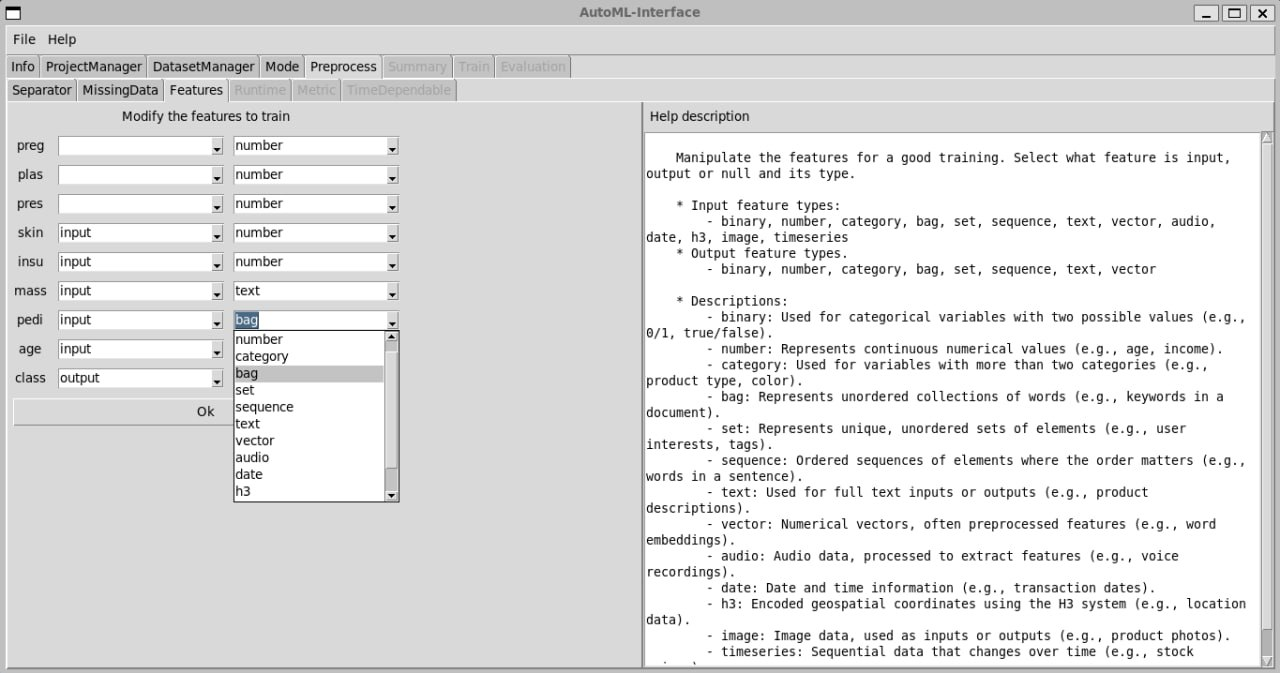
\includegraphics[width=\textwidth]{ventana preprocess features.jpg}

Tab-based navigation system that guides users
}

\headerbox{8. Conclusions}{name=conclusion,column=0,below=architecture,span=2}{

\begin{itemize} \compresslist
    \item \textbf{InsuML}: HGML implementation bridging AutoML and \textbf{non-expert users} via intuitive GUI
    \item Empirical \textbf{HCAI framework validation} on 14 OpenML datasets and assessment of\\ 13 AutoML tools
    \item \textbf{Architectural design} balancing \textbf{automation with user control}, preventing \textbf{bias} through user involvement
    \item Analysis of \textbf{performance–accessibility–transparency trade-offs}, addressing\\ ``black box'' problem 
    \item Demonstrates HGML viability when \textbf{ethics, interpretability and domain knowledge\\ integration matter alongside accuracy}
\end{itemize}

\vspace{5pt}
\textbf{Limitations}: Lower predictive performance • Requires structured tabular data • Limited explainability • Lack of user studies • Scalability challenges

\vspace{10pt}
\textbf{Future Work:} Hybrid optimization with interpretability • Automated preprocessing for heterogeneous data • Enhanced explainability (SHAP, LIME, counterfactuals) • Scalability improvements • Domain-specific workflows • Formal usability studies
}

\headerbox{Acknowledgements}{name=acknowledgements,column=2,below=gui,span=1}{
\scriptsize This work has been supported by grant PID2023-146243OB-I00 funded by MICIU/AEI/10.13039/501100011033 and by ``ERDF/EU''
}

\end{poster}

\end{document}